\section{W-mass}
\label{sec:w-mass}
With the finished calibration, the mass of the W-boson can now be measured. This is done using a the Jacobi peak of the electron transverse momentum distribution.
In order to determine the W-mass, we use a data set of actual ATLAS data containing $W \rightarrow e\nu$ events,
as well as several simulated data sets also containing $W \rightarrow e\nu$ events. 
There is also a $Z^0 \rightarrow e^+e^-$ data set to check the validity of the previous calibration.
Finally there are data sets for QCD- and non-QCD background events.

\subsection{Electron Calibration Verification}

\begin{figure}[H]
    \centering
    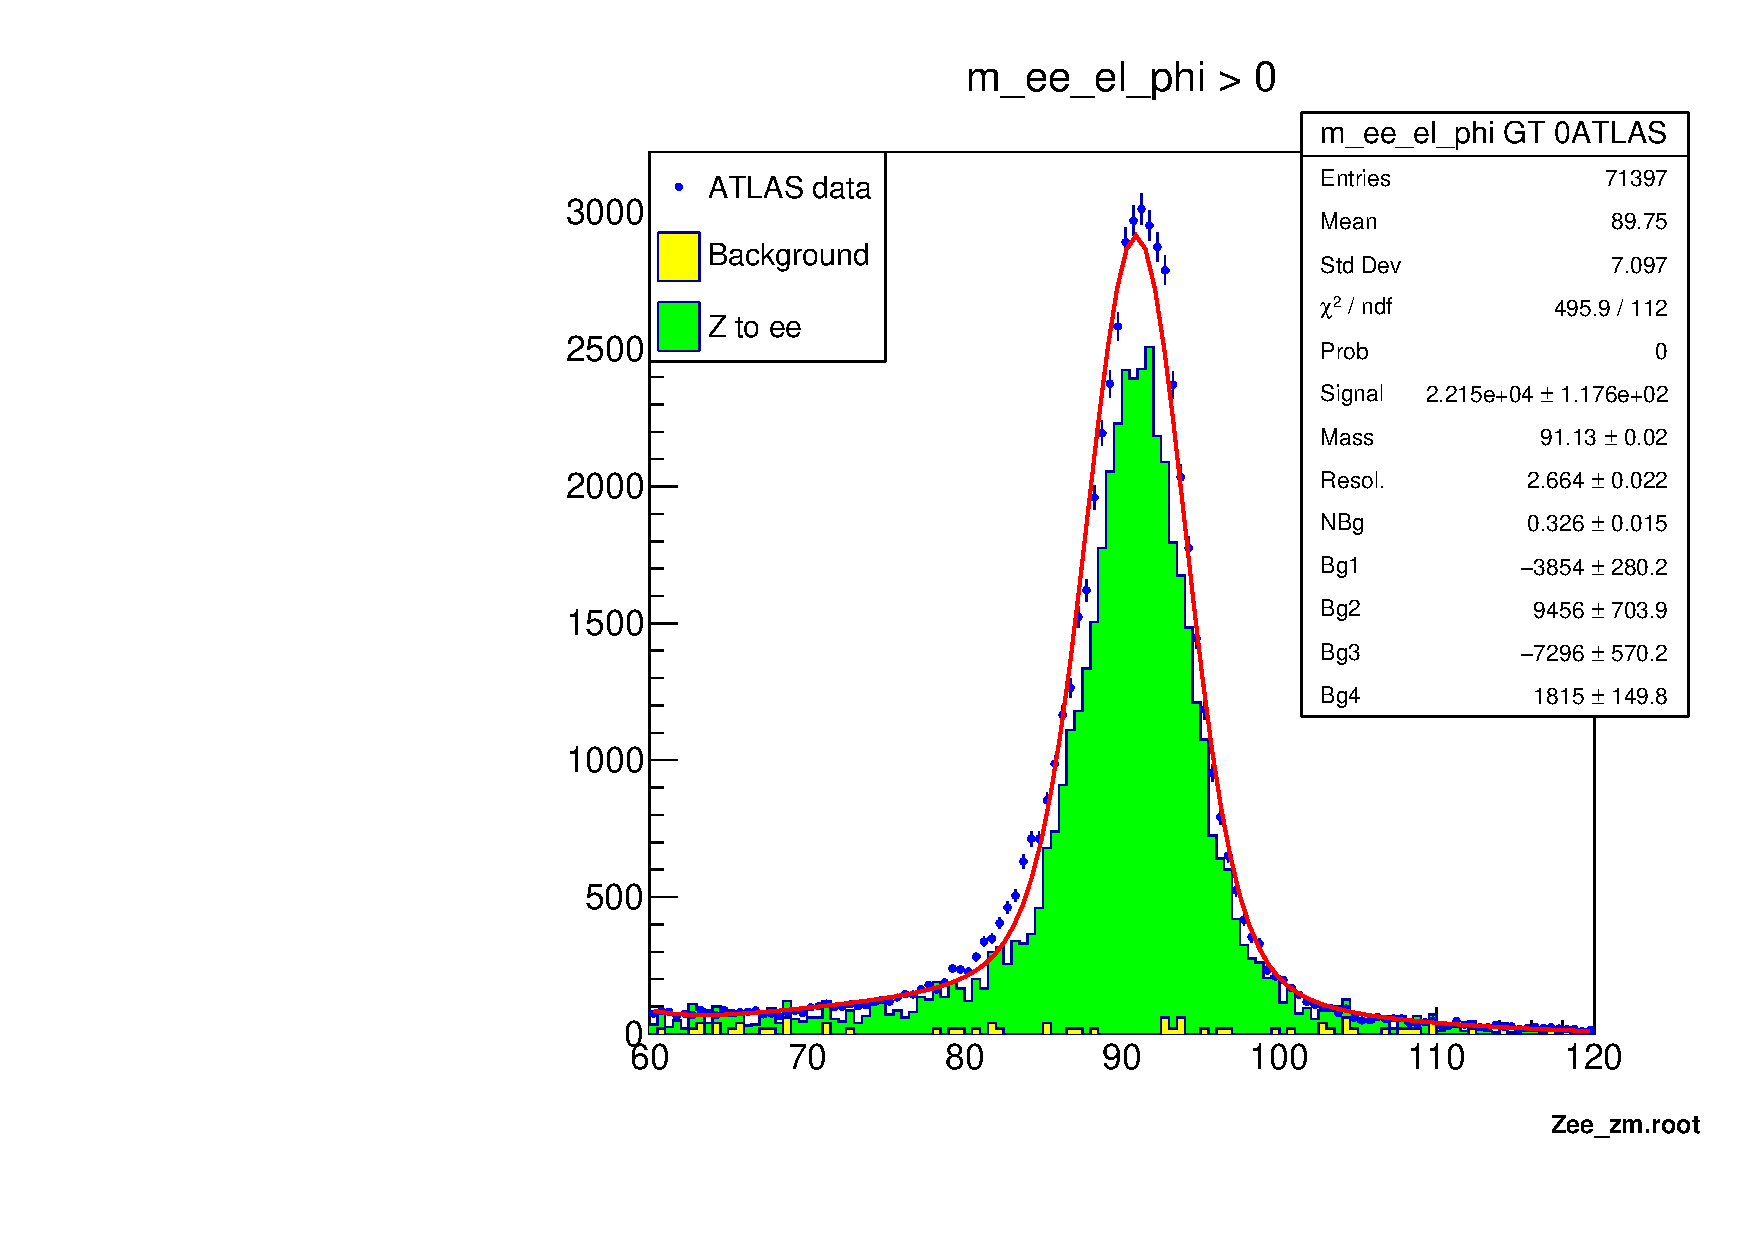
\includegraphics[width=0.7\textwidth]{../W_mass/Z_mass_check_phi_positive.pdf}
    \caption{$Z_mass_check_el_pt-cut.pdf$}
    \label{fig:z-mass_check}
\end{figure}

\begin{table}[H]
    \centering
    \begin{tabular}{ccc}
        \toprule
        \toprule
        cut selection & $M_{Z^0,meas}$ / GeV & $\bigl| \frac{M_{Z^0,meas}- M_{Z^0,lit}}{M_{Z^0,meas}} \bigr|$ \\
        \midrule
        $p_{T,e^{\pm}} > 40$ GeV & $91.71 \pm 0.02$ & \\
        $p_{T,e^{\pm}} < 40$ GeV & $90.5 \pm 0.0$ & \\
        $35 < p_{T,e^{\pm}} < 55$ GeV & $91.43 \pm 0.02$ & \\
        $\eta > 2$ & $89.89 \pm 0.05$ & \\
        $\eta < 0.5$ \& $p_{T,e^{\pm}} > 40$ & $91.69 \pm 0.02$ & \\
        $\eta < 0.5$ \& $p_{T,e^{\pm}} < 40$ & $90.56 \pm 0.03$ & \\
        $\phi < 0$ & $91.14 \pm 0.02$ & \\
        $\phi > 0$ & $91.13 \pm 0.02$ & \\
        \bottomrule
        \bottomrule
    \end{tabular}
    \caption{Measured $Z^0$ mass for different cut selections}
    \label{tab:z-masses}
\end{table}


\subsection{QCD scale factor}
In order to achieve an accurate measurement of the W-mass, the background processes at ATLAS have to be taken into consideration.
At LHC, proton proton collisions cause the measured events, therefore the background coming from QCD processes is large. This causes a problem,
since the final products of the $W \rightarrow e\nu$ events we use to measure the W-mass are leptons which do not interact with the strong interaction.
This makes the simulation of a QCD background for the $W \rightarrow e\nu$ events difficult. In order to solve this problem, the QCD background is extracted
from the data. In order to scale the data correctly, a QCD scale factor is used, since the integrated luminosity of the background is not measured and therefore
unknown. In order to get an understanding of the QCD scale factor and its effect on the data, different kinematic values are be plotted for different 
QCD scale factors.

\subsubsection{Kinematic Variables}
In order to get a feeling for the QCD scale factor and estimate its optimal value, different kinematic Variables are analyzed.
The chosen kinematic variables are $el_pt$ (the transverse momentum of the electron), etmis (missing transverse energy/momentum),
njet (number of jets in the event) and ptw (transverse momentum of the W boson). The distributions of these different variables
for a scale factor of 1 (meaning no scaling) can be seen in figure \ref{fig:qcd1}

\texttt{el\_pt}
\subsection{Cut selection}

\subsection{Gauge curves}

\subsection{W-mass }